\documentclass[12pt]{article}
\usepackage[hmargin=0.80in, vmargin=1in]{geometry}
\usepackage[T1]{fontenc}

\setlength{\topskip}{0mm}\setlength{\parskip}{1ex}\setlength{\parindent}{0mm}
\usepackage{enumitem}\setlist{nolistsep}
\usepackage[utf8]{inputenc}
\usepackage{listings}
\usepackage{grffile}


\usepackage{fancyhdr}\pagestyle{fancy}
\lhead{\today}\chead{{\bf DIKU - AADS - Assignment 1 - 2017}}\rhead{Jan Sokol, Denis Trebula}

\usepackage{lastpage}
\usepackage{graphicx}
\cfoot{Page \thepage\ }

\begin{document}

\newcommand{\topic}[1]{
  \begin{minipage}{\linewidth}
  {\bf #1}

  \end{minipage}
}
 Jan Sokol - kgj360 || Denis Trebula \\


\topic{1. Hash functions for sampling}

(a) Prove that $p \leq Pr[hm(x)/m < p] \leq 1.01p $. For this we will use few things. 

$ h(x) = h_m(x)/m $ is Strong Independent Hash Function; \\
$ p \geq 100/m  \Rightarrow p/100 \geq 1/m$; \\
$ hm(x)/m \leq p \Rightarrow hm(x) \leq mp$; \\

\begin{lstlisting}[language=R]
\end{lstlisting}


(b)

\topic{2. Bottom-k sampling}


Prove that $ E[|C \cap S_h^k(A)|/k] = |C |/|A| $, assuming that $ S_h^k(A) $is a uniformly random size-k $ \subset	A$.

We assume that $C \subset	A$ and $S_h^k(A) \subset	A$ are independent, as shown on Venn diagram bellow:

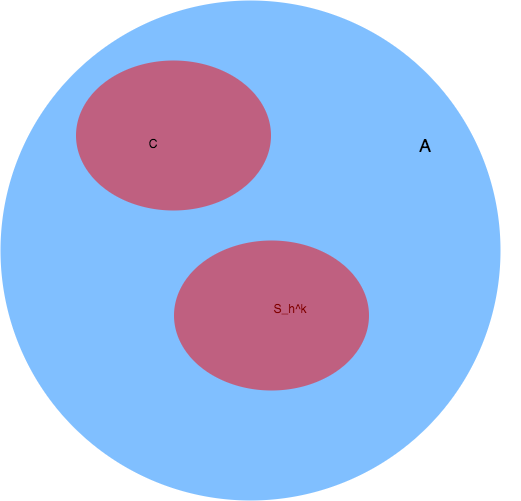
\includegraphics[scale=0.3]{venn.png}

Seeing this we can say:

$Pr[x \in S_h^k(A)] = \frac{k}{|A|} $ \\
$Pr[x \in C] = \frac{C}{|A|} $\\

$  E[|C \cap S_h^k(A)|/k] $ \\
$= \frac{1}{k} E[|C \cap S_h^k(A)|] $ \\
$= \frac{1}{k}  \sum_{\forall a \in A}  E[a \in C \wedge a \in S_h^k(A)] $ \\
$= \frac{1}{k}  \sum_{\forall a \in A}  Pr[a \in C \wedge a \in S_h^k(A)] $ \\
$= \frac{1}{k}  \sum_{\forall a \in A}  Pr[a \in C] \cdot Pr[a \in S_h^k(A)] $ 				\hfill	(From independence)\\
$= \frac{1}{k}  \sum_{\forall a \in A}  (\frac{C}{|A|} \cdot \frac{k}{|A|} )] $ 			\hfill	(Substitution from above)\\
$= \frac{1}{k}  \sum_{\forall a \in A}  (\frac{C}{|A|} \cdot \frac{k}{|A|} ) $ 			\hfill	(Substitution from above)\\
$= \frac{1}{k} \frac{C}{|A|} \cdot \frac{k}{|A|} \sum_{\forall a \in A}  1 $ 			\hfill	(Elements in sum are not dependant on $a \in A$)\\
$= \frac{1}{k} \frac{C}{|A|} \cdot \frac{k}{|A|} |A| $ 			\hfill	\\
$= \frac{C}{|A|} $ 			\hfill	\\

\topic{2.1 Frequency estimation}

Exercise 2

(a) As a data structure we would use binary heap (max heap). Binary heaps are a one of the ways of implementing priority queues. In the heap we would only store k smallest keys.

(b) To process another key from the stream it would take $ O(log_2 k)$.

\topic{2.2 Similarity estimation}

(a)

(b)

(c)

\topic{3 Bottom-k sampling with strong universality}

\topic{3.1 A union bound}

exercise 5

\topic{3.2 Upper bound with 2-independence}

exercise 6

exercise 7

\end{document}
